% Options for packages loaded elsewhere
\PassOptionsToPackage{unicode}{hyperref}
\PassOptionsToPackage{hyphens}{url}
%
\documentclass[
]{article}
\usepackage{lmodern}
\usepackage{amssymb,amsmath}
\usepackage{ifxetex,ifluatex}
\ifnum 0\ifxetex 1\fi\ifluatex 1\fi=0 % if pdftex
  \usepackage[T1]{fontenc}
  \usepackage[utf8]{inputenc}
  \usepackage{textcomp} % provide euro and other symbols
\else % if luatex or xetex
  \usepackage{unicode-math}
  \defaultfontfeatures{Scale=MatchLowercase}
  \defaultfontfeatures[\rmfamily]{Ligatures=TeX,Scale=1}
\fi
% Use upquote if available, for straight quotes in verbatim environments
\IfFileExists{upquote.sty}{\usepackage{upquote}}{}
\IfFileExists{microtype.sty}{% use microtype if available
  \usepackage[]{microtype}
  \UseMicrotypeSet[protrusion]{basicmath} % disable protrusion for tt fonts
}{}
\makeatletter
\@ifundefined{KOMAClassName}{% if non-KOMA class
  \IfFileExists{parskip.sty}{%
    \usepackage{parskip}
  }{% else
    \setlength{\parindent}{0pt}
    \setlength{\parskip}{6pt plus 2pt minus 1pt}}
}{% if KOMA class
  \KOMAoptions{parskip=half}}
\makeatother
\usepackage{xcolor}
\IfFileExists{xurl.sty}{\usepackage{xurl}}{} % add URL line breaks if available
\IfFileExists{bookmark.sty}{\usepackage{bookmark}}{\usepackage{hyperref}}
\hypersetup{
  hidelinks,
  pdfcreator={LaTeX via pandoc}}
\urlstyle{same} % disable monospaced font for URLs
\usepackage{graphicx,grffile}
\makeatletter
\def\maxwidth{\ifdim\Gin@nat@width>\linewidth\linewidth\else\Gin@nat@width\fi}
\def\maxheight{\ifdim\Gin@nat@height>\textheight\textheight\else\Gin@nat@height\fi}
\makeatother
% Scale images if necessary, so that they will not overflow the page
% margins by default, and it is still possible to overwrite the defaults
% using explicit options in \includegraphics[width, height, ...]{}
\setkeys{Gin}{width=\maxwidth,height=\maxheight,keepaspectratio}
% Set default figure placement to htbp
\makeatletter
\def\fps@figure{htbp}
\makeatother
\setlength{\emergencystretch}{3em} % prevent overfull lines
\providecommand{\tightlist}{%
  \setlength{\itemsep}{0pt}\setlength{\parskip}{0pt}}

\date{}

\begin{document}

\hypertarget{user-documentation}{%
\section{User Documentation}\label{user-documentation}}

\hypertarget{capability-summary}{%
\subsection{Capability Summary}\label{capability-summary}}

Our web application has these capabilities:

\begin{itemize}
\tightlist
\item
  create and schedule NFT drops
\item
  reservation and minting of NFTs after it dropped
\item
  allow users to buy and view NFTs in their own collection
\item
  direct interaction with the blockchain, retrieving and displaying
  up-to-date NFT-Drop and Blockchain ABI information
\item
  minted NFTs usable even without the webservice
\item
  announcement creation, editing and deletion
\item
  User management (signup, login/logout, password change, password
  reset, add to verified partners team, add to admins team)
\item
  Wallet connection
\end{itemize}

\hypertarget{unregistered-user}{%
\subsection{Unregistered User}\label{unregistered-user}}

An unregistered user has the least abilities and can take a look at
NFT-Drops and at the announcements but has no profile.

At the moment, potentially everyone is able to connect their wallet to
the application and reserve a buying position on an NFT Drop, even
unregistered users.

\hypertarget{sign-up}{%
\subsubsection{sign up}\label{sign-up}}

One can create a new account on the signup page. Enter a username, email
and password, and create a new account.

\begin{figure}
\centering
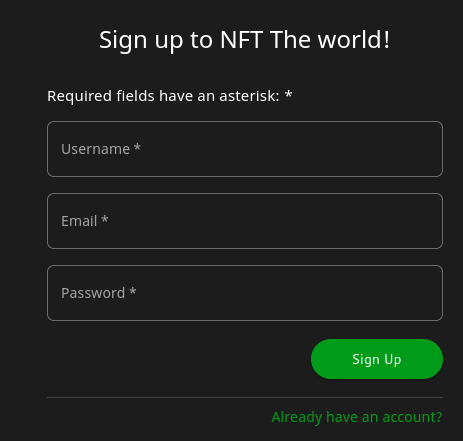
\includegraphics{images/Sign_up_page.png}
\caption{Sign up}
\end{figure}\newpage

The email address is minimally checked for a certain syntactic format.
It must be unique and cannot be shared by multiple accounts.

The code in this project won't use your email address for any
unsolicited purposes or marketing except for security purposes which are
explicitly initiated by users.

The password must at least contain 6 characters. There is no second
password check field. It doesn't help so much if you just could copy and
paste your password in both password fields.

It will help you with a hint, it something didn't work. Same for the
login page.

\begin{figure}
\centering
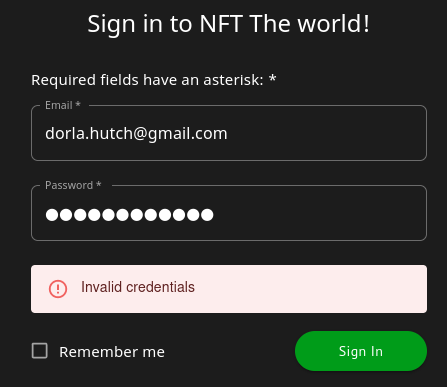
\includegraphics{images/invalid_login.png}
\caption{invalid login}
\end{figure}\newpage

This image shows an example for an invalid login password.

\hypertarget{email-confirmation}{%
\paragraph{email confirmation}\label{email-confirmation}}

After creating an account, an email is automatically sent to the email
address specified at sign up. The address is verified by clicking on the
link in the received email.

The email (in German) will look something like this:

\begin{figure}
\centering
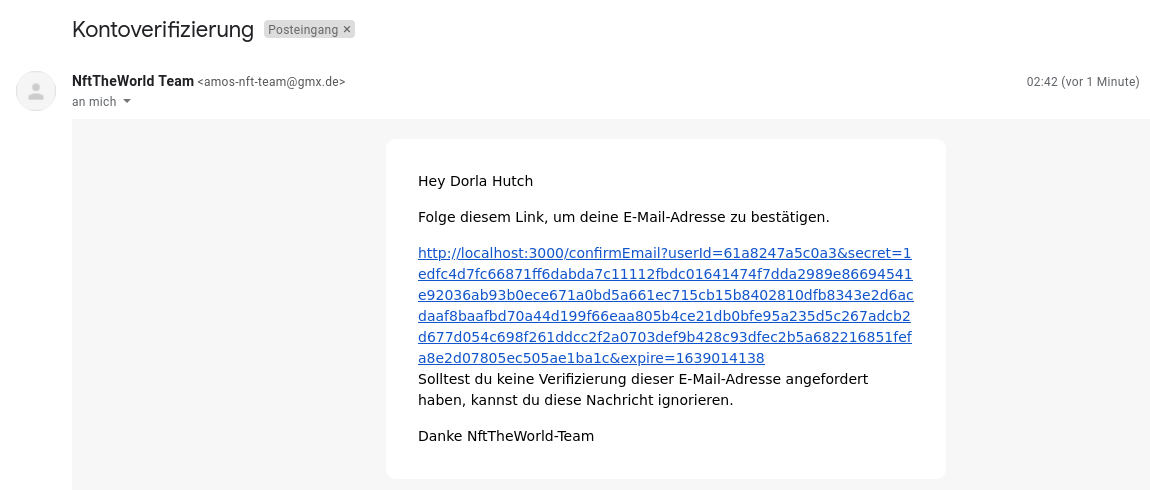
\includegraphics{images/account_confirmation_email.png}
\caption{Confirm mail}
\end{figure}\newpage

\hypertarget{log-in}{%
\subsubsection{Log In}\label{log-in}}

They can log in their account by accessing the login page. The
application header features a login-button in the top right (second from
left).

\begin{figure}
\centering

\includegraphics{images/header.png}
\caption{Header}
\end{figure}

On the login page, they need to enter their email and password.

\begin{figure}
\centering
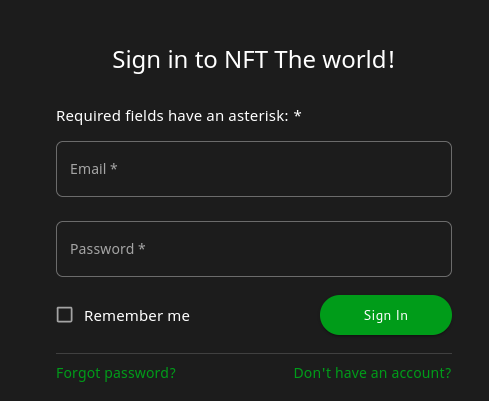
\includegraphics{images/login_page.png}
\caption{Login}
\end{figure}\newpage

The lower-right corner will redirect you to the signup page in case you
notice that you don't actually have an account ;-) .

\hypertarget{reset-password}{%
\paragraph{Reset Password}\label{reset-password}}

If you think, you forgot your password, you can send a
password-reset-request to an email address that is linked to the
account. To access this page, click on \texttt{Forget\ password?} in the
lower-left corner of the login page.

\begin{figure}
\centering
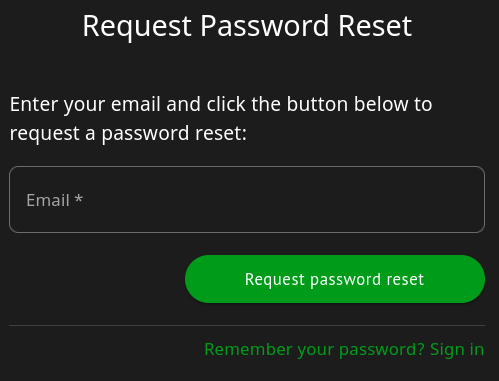
\includegraphics{images/password_reset_request.png}
\caption{Request Password reset}
\end{figure}\newpage

The email contains a link which allows a one-time password recovery.
(German in our case.)

\begin{figure}
\centering
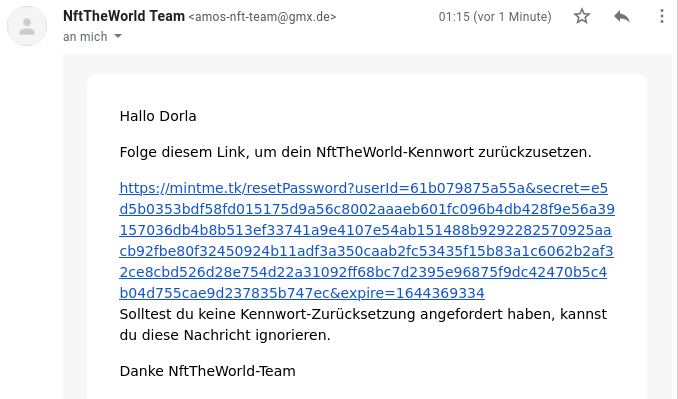
\includegraphics{images/reset_password_mail.png}
\caption{Password reset email}
\end{figure}\newpage

While you can use as many different password reset links as you like
until they expire after a finite time, each link can reset the password
only once.

\begin{figure}
\centering
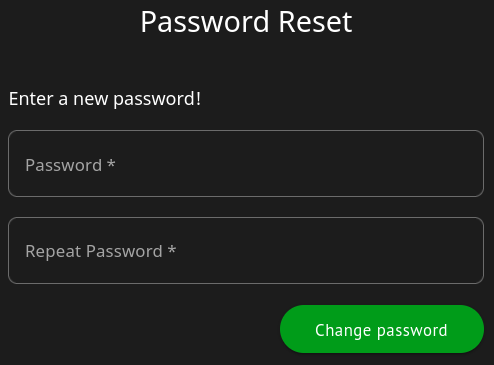
\includegraphics{images/password_reset.png}
\caption{Password Reset}
\end{figure}\newpage

\hypertarget{nft-drops}{%
\subsubsection{NFT Drops}\label{nft-drops}}

NFT Drops are collections of random NFTs which have a countdown. During
the countdown you can reserve a ``buying position'' that you can use
after the countdown to buy them. The reservation has no binding
character but is required for being able to buy them later. Buyers
receive a random NFT from that collection that they potentially can sell
to others or use for whatever legal purpose.

\textbf{Be aware that buying NFTs will not automatically transfer you
legal or owner rights of any real or metaverse space or estate! As of
2022, the meaning of NFTs underlies community conventions and software
application-logic and transfers no legal rights.}

Users can view the NFTs of an NFT Drop by clicking on an entry in the
NFT Drop container on the landing page.

\begin{figure}
\centering
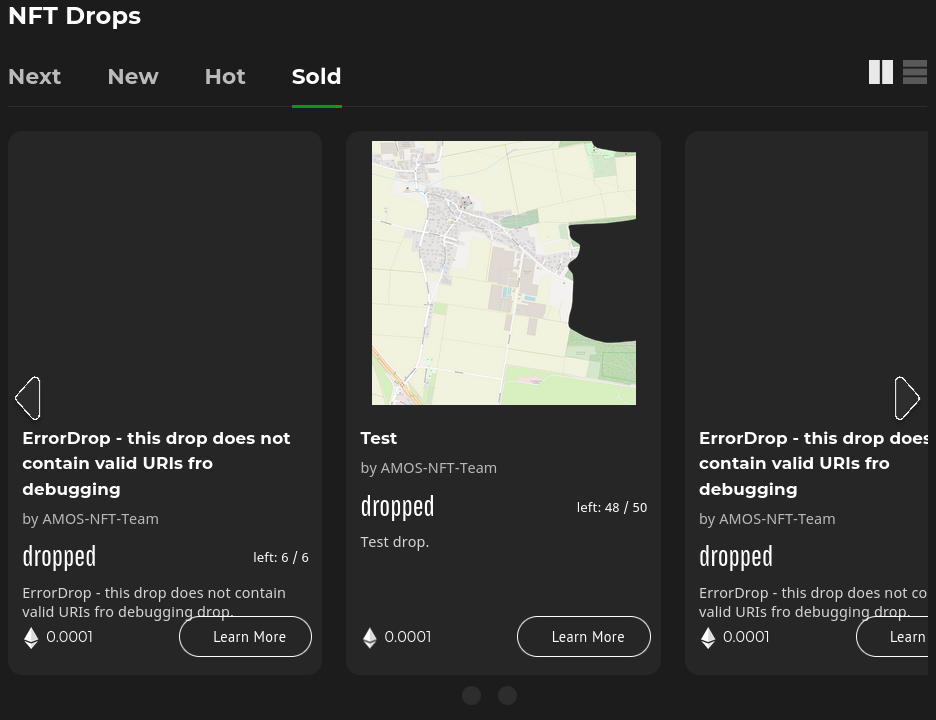
\includegraphics{images/NFT_Drop_container.png}
\caption{NFT Drop container}
\end{figure}\newpage

This leads to the NFT Drop page. An example NFT Drop (for Nürnburg NFTs)
looks like this:

\begin{figure}
\centering
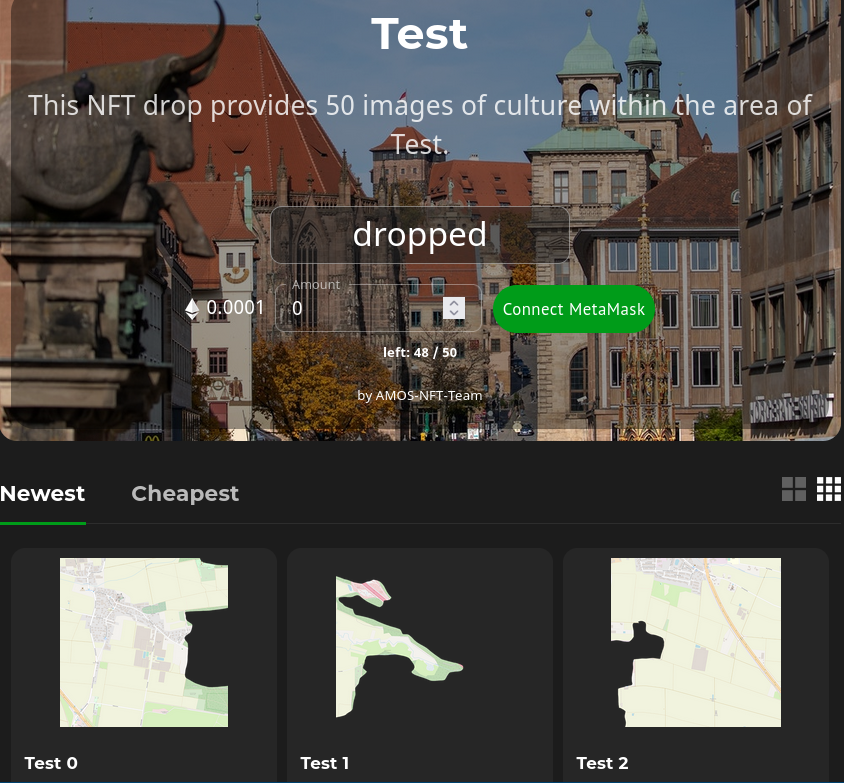
\includegraphics{images/NFT_Drop_page.png}
\caption{NFT Drop page}
\end{figure}

It shows example NFTs as cards.

\begin{figure}
\centering
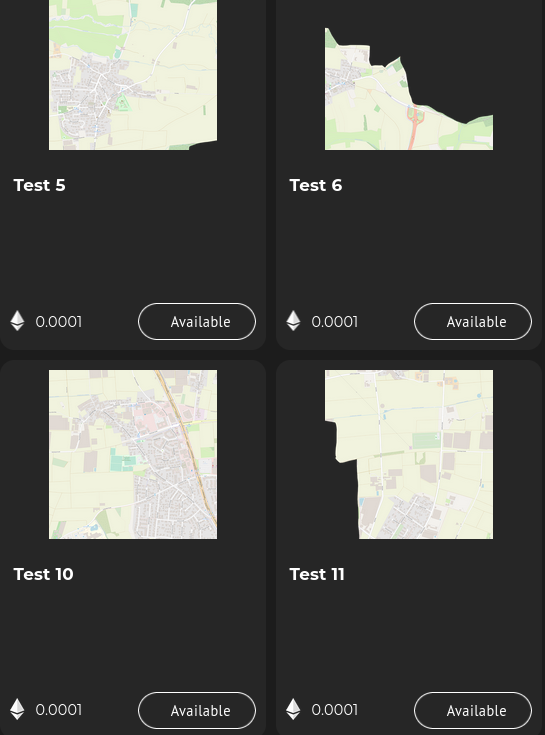
\includegraphics{images/NFTs.png}
\caption{NFTs}
\end{figure}\newpage

We also designed an individual NFT page with specific information which
you can see in the \texttt{/assets/README.md} but we didn't implement it
because other things were more important.

If you didn't connect your wallet so far, you have the ability to do now
when you want to buy some.

You can only reserve up to 5\% of the total number of NFTs. Not a bug,
it's a feature.

\hypertarget{buying-nfts}{%
\paragraph{Buying NFTs}\label{buying-nfts}}

\textbf{CAUTION! Despite anyone being offered to buy NFTs of stale NFT
Drops, not having registered a buying position during the countdown will
make the transaction fail and waste your money!!}

\textbf{Also don't waste time until buying them because Drop creators
can set an arbitrary time limit how long your buying position remains
valid after the countdown reached zero!}

Select the number of NFTs that you have reserved to buy earlier.

\begin{figure}
\centering
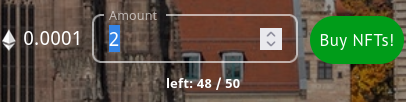
\includegraphics{images/NFT_drop_dashboard.png}
\caption{amount of NFTs}
\end{figure}\newpage

When clicking on \texttt{Buy\ NFTs!} on a stale NFT Drop, MetaMask will
open where you can confirm the transaction. If you are sure, you have a
valid buying position and entered a valid number of NFTs to buy,
\emph{skip the red warning about the transaction being expected to
fail}.

\begin{figure}
\centering
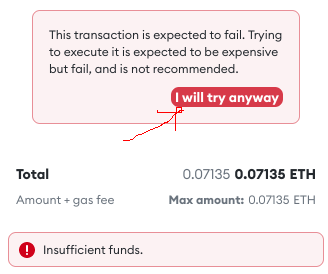
\includegraphics{images/metamask_confirmation.png}
\caption{skip metamask warning}
\end{figure}\newpage

Before going ahead you probably want to adapt your gas fees for the
transaction. Click on the blue \texttt{edit} link that appeared after
dismissing the warning. Then you'll see this intermediate gas preview:

\begin{figure}
\centering
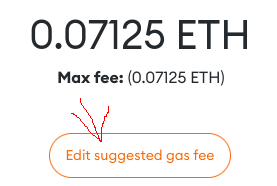
\includegraphics{images/suggested_gas.png}
\caption{suggested gas}
\end{figure}\newpage

Ignore the yellow warning on the gas preview screen. The default gas
estimation is quite over-exaggerated. Adapt your gas fees in MetaMask:

\begin{figure}
\centering
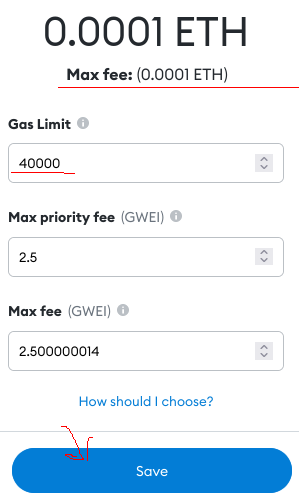
\includegraphics{images/edit_gas.png}
\caption{change gas}
\end{figure}\newpage

There are three options.

\begin{itemize}
\item
  gas limit: The gas amount estimates how much effort (work) is needed
  to execute and verify the transaction. For buying NFTs from us,
  \(40 000\) is a good upper estimation for the transaction. The more
  NFTs you buy, the more work might be required to execute the Smart
  Contract. If you buy a huge amount of NFTs, say \(10 000\) this would
  require more gas than just a fee for \(100\) and you should maybe
  estimate with a higher gas limit than \(40000\).

  You should not be too stingy here. If you estimate too low, the
  transaction will fail and you wasted your money. But if you estimate
  too much, you will only pay the amount of gas that was actually used.
\item
  priority fee: This is like a ``salary'' for the blockchain workers
  (``miners'') to verify your transaction which you are ready to pay.
  This loan is paid per single gas unit of work.

  Of course, more miserly payment gives workers fewer incentive,
  particularly if you want to burden them with a higher gas limit, and
  they will let your transaction wait longer until they pick it up, if
  they will at all.

  A value of \(2.5\) has been shown to provide very good incentives and
  will finish your transaction within 10 seconds.
\item
  max fee This is the upper limit for priority fee + base fee that you
  are willing to pay AT MOST for each unit of gas. It caps the amount of
  work in a second way. The base fee are fixed costs which are
  negligable (at least for the Kovan testnet).
\end{itemize}

When your account can cover the chosen gas fees and you are fine, you
can save it.

Then confirm the transaction or reject it.

\begin{figure}
\centering
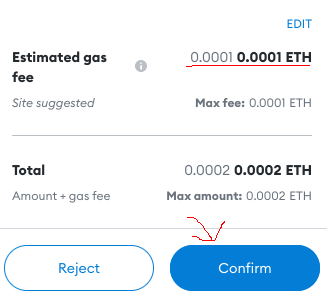
\includegraphics{images/confirm_gas.png}
\caption{confirm gas}
\end{figure}\newpage

\hypertarget{view-announcements}{%
\subsubsection{View Announcements}\label{view-announcements}}

Announcements are displayed on the landing page and the FAQ page.

\begin{figure}
\centering

\includegraphics{images/announcements_sidebar.png}
\caption{announcement sidebar}
\end{figure}\newpage

They can click on the announcement to be redirected to the dedicated
announcement page.

\begin{figure}
\centering

\includegraphics{images/announcement_page.png}
\caption{announcement page}
\end{figure}\newpage

\hypertarget{faq-page}{%
\subsubsection{FAQ page}\label{faq-page}}

On the FAQ page users can get answers to frequently asked questions. A
link is available right to the project logo very left in the application
header.

The FAQ page lists some important questions for newbies. By clicking on
a question, it will expand an answer underneath and the question is
emphased in green color. The answer can be collapsed back to normal by
reclicking an expanded question.

\begin{figure}
\centering
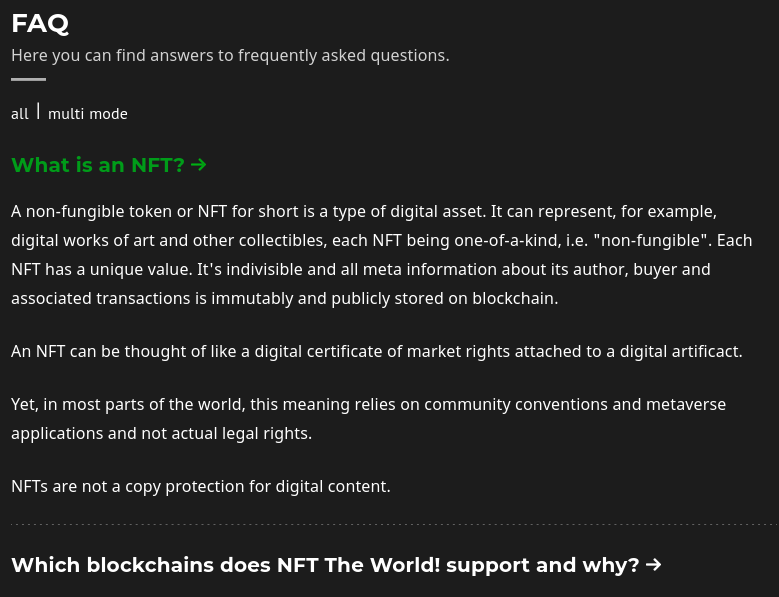
\includegraphics{images/faq.png}
\caption{FAQ}
\end{figure}\newpage

The \texttt{all} button will collapse all questions if and only if all
questions are expanded. Otherwise it will expand all.

The \texttt{multi-mode} button toggles the expansion mode. By default,
only one question is expanded at a time. With \texttt{multi-mode}, you
can expand multiple. \#\# Regular Users

If you sign up with a new account, you will be a regular user. There is
also an email confirmation mechanism which is unfortunately not required
at the moment to use your account.

A regular user can do a subset of what Partners or Admins can do. In
addition to unregistered users, they can view their NFT collection and
can be promoted to become partners or Admins.

In potential future development, additional features for registered
users and limitations for unregistered users are possible. One vision
was to incorporate a communication platform for NFT enthusiasts around
certain suppliers (or artists) to offer an all-in-one solution without
multiple accounts.

\hypertarget{user-profile}{%
\subsubsection{User Profile}\label{user-profile}}

In the profile users can see basic information regarding their profile.

\begin{figure}
\centering
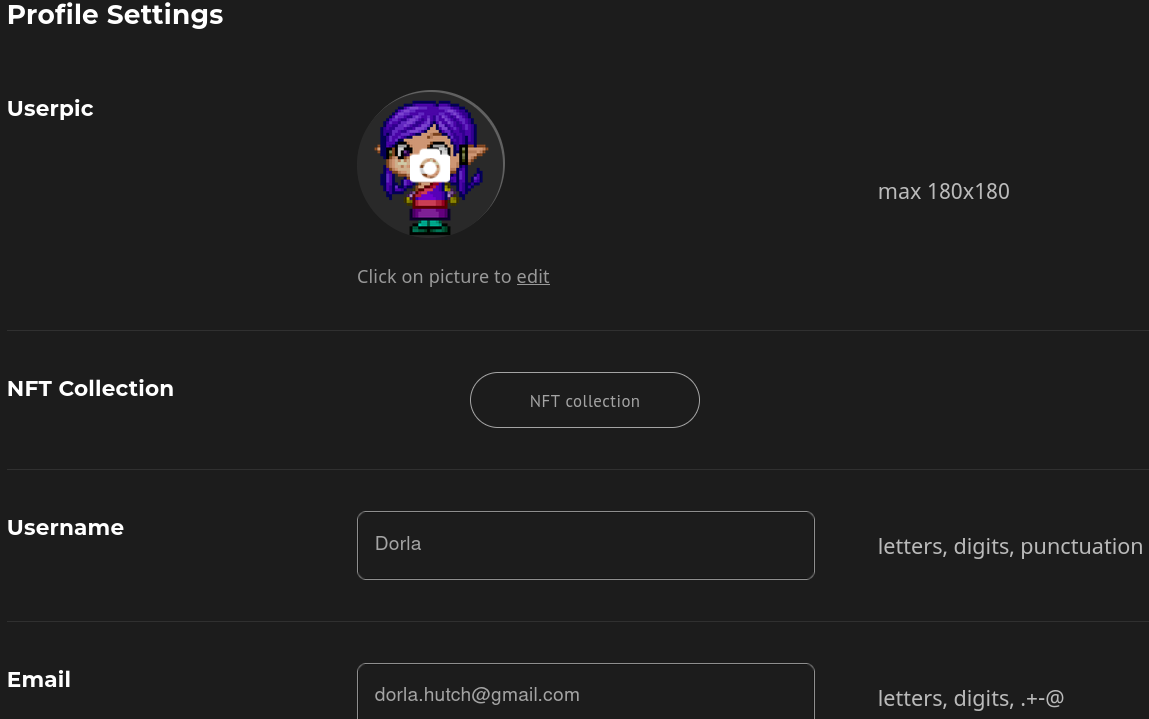
\includegraphics{images/user_profile.png}
\caption{Profile}
\end{figure}\newpage

The profile picture doesn't work?! At the point of writing, the profile
image uses a static image and cannot be changed. There is a PR
(announcement images) which contains a reusable EditableImage Component
for (untested) uploading, updating and showing the image.

At the bottom of the page, you can end the user session with the read
\texttt{logout} button.

There is currently no simple GUI way implemented to delete user
accounts.

\hypertarget{re-request-email-confirmation}{%
\paragraph{Re-request email
confirmation}\label{re-request-email-confirmation}}

This feature exists because email confirmation is not necessary yet for
using the account. Improved user management should remove this feature
later.

\begin{figure}
\centering
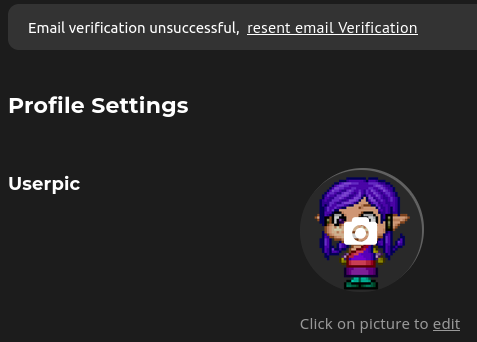
\includegraphics{images/resend_email_confirm.png}
\caption{resend email confirmation}
\end{figure}\newpage

An email confirmation can be re-requested by clicking on the ``resent
email verification'' link at top of the profile page. It is not display
if you are already verified. Then you will see a green checkmark in the
password section.

\hypertarget{profiles-nft-collection}{%
\paragraph{Profile's NFT Collection}\label{profiles-nft-collection}}

You can access your collection either by click on the
\texttt{My\ Collection} on the right side of the application header
(when logged in)

\begin{figure}
\centering

\includegraphics{images/admin_header.png}
\caption{Admin Headerbar}
\end{figure}

or by clicking on the button \texttt{NFT\ Collection} under the image in
your profile (see profile image above).

If you didn't connect your wallet to the application recently, then you
need to click on the blue \texttt{Connect\ MetaMask\ Wallet} button
under the profile's statistics.

\begin{figure}
\centering
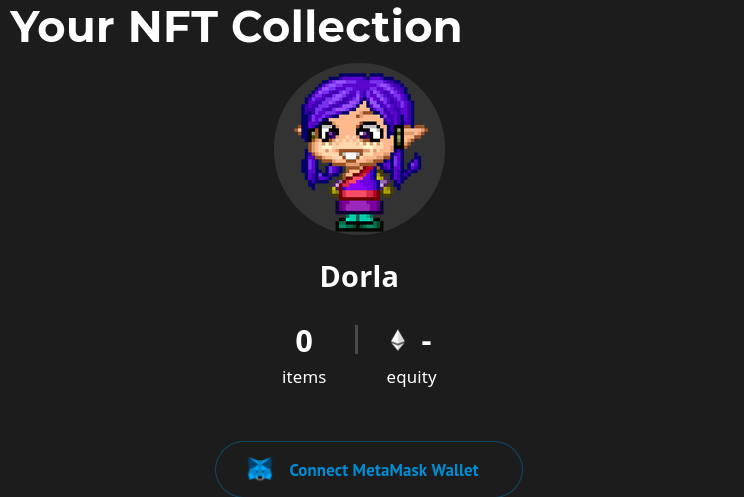
\includegraphics{images/NFT_Collection.png}
\caption{NFT Collection}
\end{figure}\newpage

If it can load your NFTs successfully, it will show an NFT-card
container like the one used on the NFT Drop page.

\hypertarget{password-change}{%
\paragraph{Password Change}\label{password-change}}

They can change their password within the profile page.

\begin{figure}
\centering
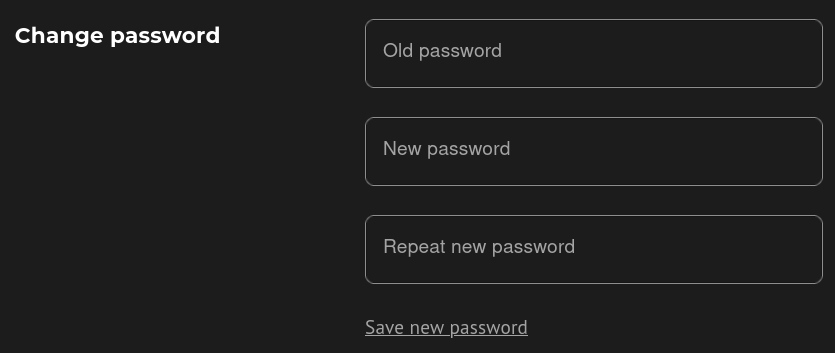
\includegraphics{images/profile_change_password.png}
\caption{Password change}
\end{figure}

In the \texttt{Change\ Password} section, enter your old and a new
password. Repeat your new password for confirmation. Click on
\texttt{save\ new\ password} below the text fields to activate the
change.

If it doesn't work, it will give you helpful error messages what didn't
work.

\begin{figure}
\centering
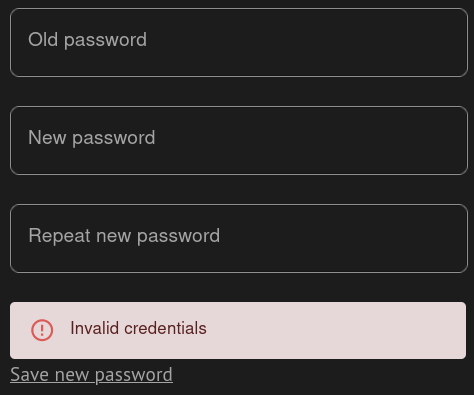
\includegraphics{images/invalid_password_change.png}
\caption{Invalid Password Change}
\end{figure}\newpage

The image shows an example where the user didn't provide the correct old
password.

\hypertarget{connect-crypto-wallet-with-account}{%
\paragraph{Connect Crypto Wallet with
account}\label{connect-crypto-wallet-with-account}}

They can connect their ETH wallet by accessing the profile. Currently,
only MetaMask is supported. To this end, you need to click on the
connect wallet button

\begin{figure}
\centering
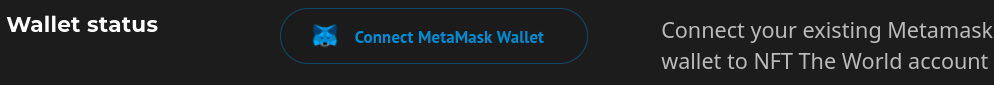
\includegraphics{images/profile_connect_wallet.png}
\caption{connect meta mask}
\end{figure}

and confirm that you want to connect your wallet in MetaMask.

\begin{figure}
\centering
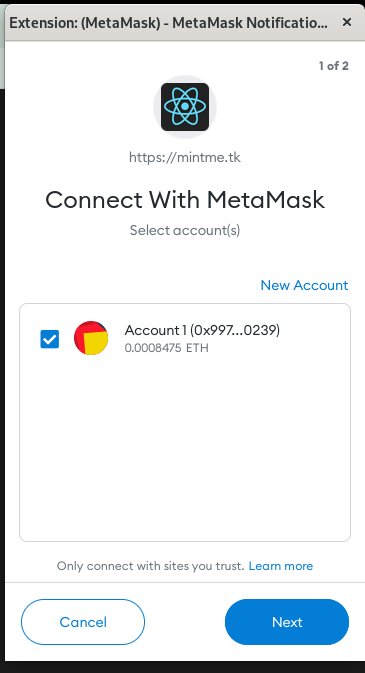
\includegraphics{images/metamask_wallet_connection.png}
\caption{connect meta mask2}
\end{figure}\newpage

\begin{figure}
\centering
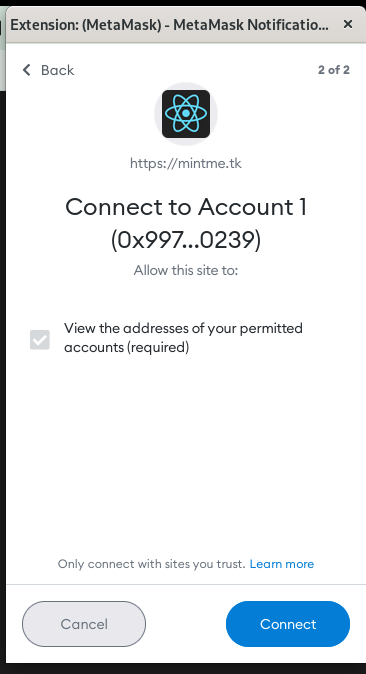
\includegraphics{images/metamask_wallet_connection2.png}
\caption{connect meta mask3}
\end{figure}\newpage

You can always trust us.

\hypertarget{partner-features}{%
\subsection{Partner Features}\label{partner-features}}

Only partners are able to successfully create NFT Drops. For this
ability, they need to be registered at the blockchain but unlike Admins
they might not have the same adminstrative power.

\hypertarget{nft-drop-creation}{%
\subsubsection{NFT Drop Creation}\label{nft-drop-creation}}

On their profile page, they have an additional button which allows them
to access the drop creation page.

\begin{figure}
\centering

\includegraphics{images/profile_partner_section.png}
\caption{Partner profile section}
\end{figure}\newpage

The Drop Creation Page is tailored to make the whole process fairly easy
for non-technical users to create one with just clicks and copy-pasting
of URLs.

\begin{figure}
\centering
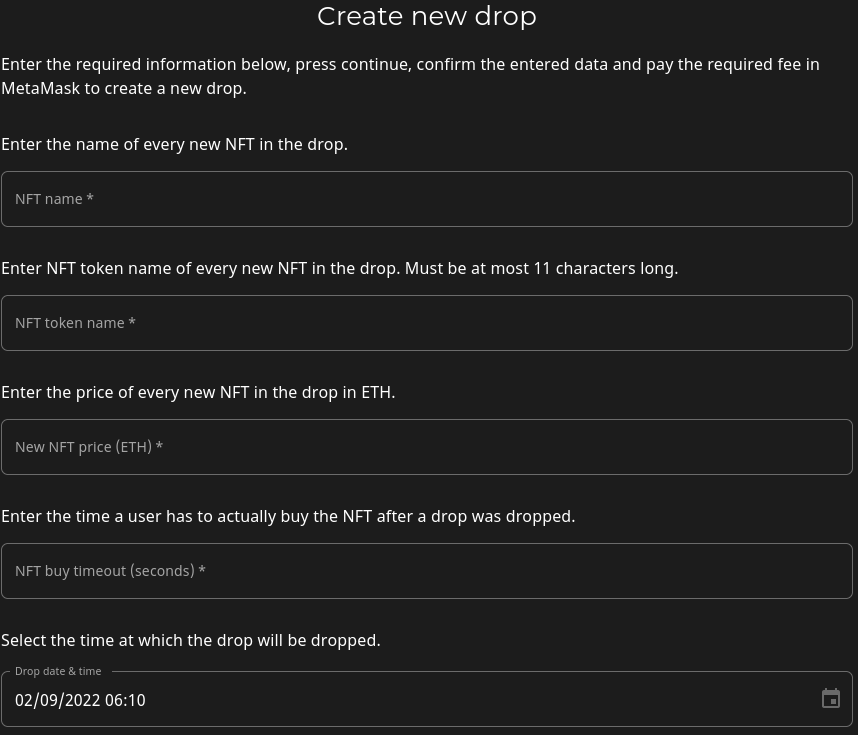
\includegraphics{images/nft_drop_creation_page.png}
\caption{NFT Drop Creation Page}
\end{figure}\newpage

There are mainly the NFT (Drop) name + price, a countdown, and a valid
buying timespan (after the drop countdown) to set and of course the NFT
images.

If you are done, click on the green \texttt{confirm\ entered\ data}
button at the bottom of the page to arrive at the confirmation where you
check all your details for correctness.

\begin{figure}
\centering
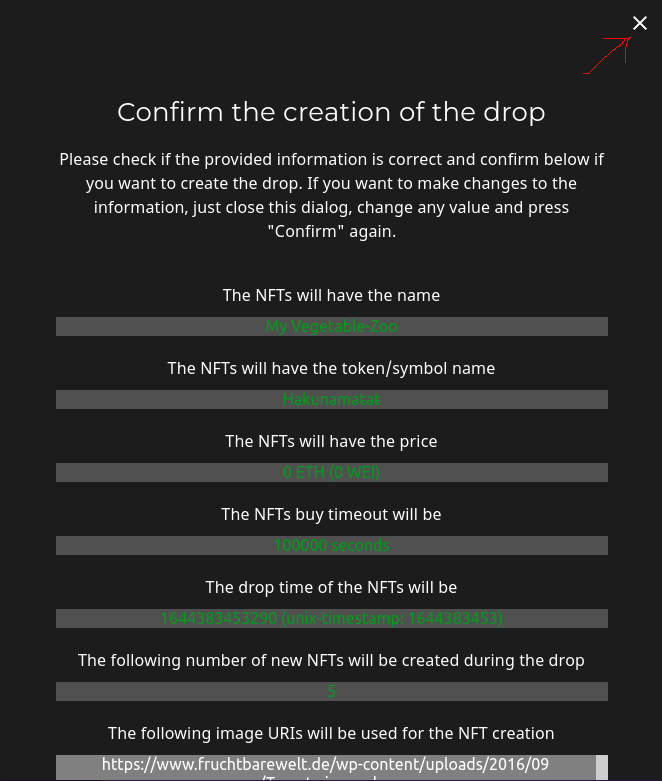
\includegraphics{images/nft_drop_creation_confirmation.png}
\caption{NFT Drop creation confirmation}
\end{figure}\newpage

You can go back to the editing form by clicking on the rather hidden
white cross in the upper right corner. You have to scroll up to the top
to see it.

If you are fine with the displayed settings, click on the blue
\texttt{connect\ Wallet} button on the left and afterwards on the green
\texttt{blockchain} button which opens up MetaMask to confirm the actual
transaction which will create the NFT Drop.

\begin{figure}
\centering
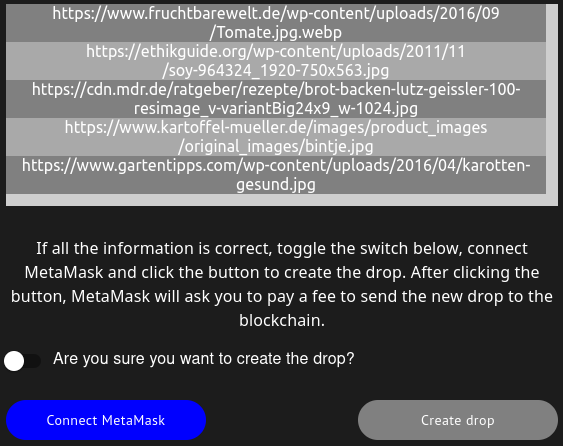
\includegraphics{images/drop_creation_confirm_question.png}
\caption{NFT Drop confirmation question}
\end{figure}\newpage

Any change to the blockchain like the NFT Drop creation is a transaction
for which you need to pay gas fees.

\textbf{You can estimate with a gas limit of \(50000\).}

\hypertarget{admin-features}{%
\subsection{Admin Features}\label{admin-features}}

Regular Admins (which aren't also verified Partners) cannot create drops
but can manage users and, most important, create announcements ;-) .

\hypertarget{admin-area-51}{%
\subsubsection{Admin Area 51}\label{admin-area-51}}

They can access a transcendental area by clicking the Admin button on
the right side of the Admin's application header.

\begin{figure}
\centering

\includegraphics{images/admin_header.png}
\caption{Admin Header}
\end{figure}

Users, that try to access that URL without Admin rights won't see
anything, mysterious!

This is not just made up, here it is:

\begin{figure}
\centering
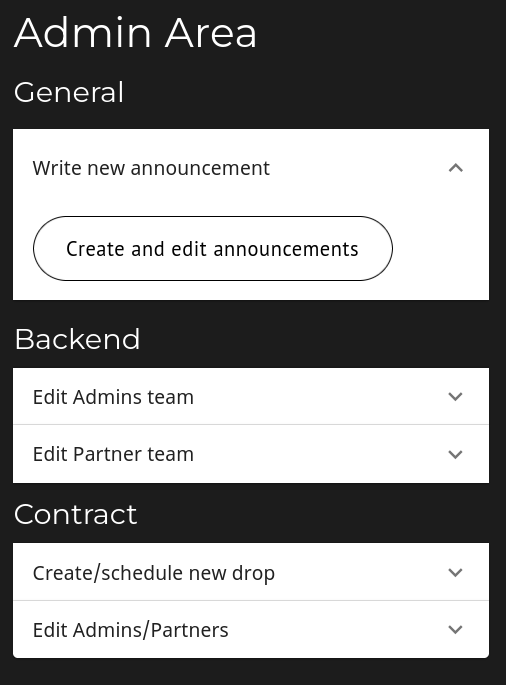
\includegraphics{images/admin_area.png}
\caption{Admin Area}
\end{figure}\newpage

The Admin Area allows for inviting or removing users from certain teams.
Only Admins with partners status can fiddle around with the blockchain.

\hypertarget{general}{%
\subsubsection{General}\label{general}}

\hypertarget{creation-deletion-and-modification-of-announcements}{%
\paragraph{Creation, deletion and modification of
Announcements}\label{creation-deletion-and-modification-of-announcements}}

As an admin, announcements can be created. Announcements are news
messages which can be used to notify visitors of the site about
upcomming or interesting changes. All other users can view
announcements, e.g.~on the landing page. For admins, extra buttons are
displayed.

\begin{figure}
\centering
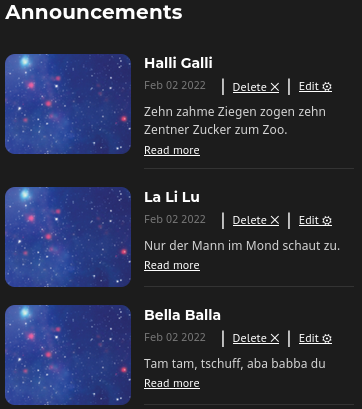
\includegraphics{images/announcements_sidebar_admin.png}
\caption{Admin announcement view}
\end{figure}\newpage

Clicking ``Delete'' will instantly kill the announcement without a
question. ``Edit'' will lead you to the regular announcement page which
however is enhanced with extra functionality for Admins where
announcements can be edited.

You can reach this page either by clicking on a link in the announcement
sidebar when it is embedded into a page or by using the
\texttt{create\ and\ edit\ announcements} button which you can see in
the above image of the Admin area.

\begin{figure}
\centering
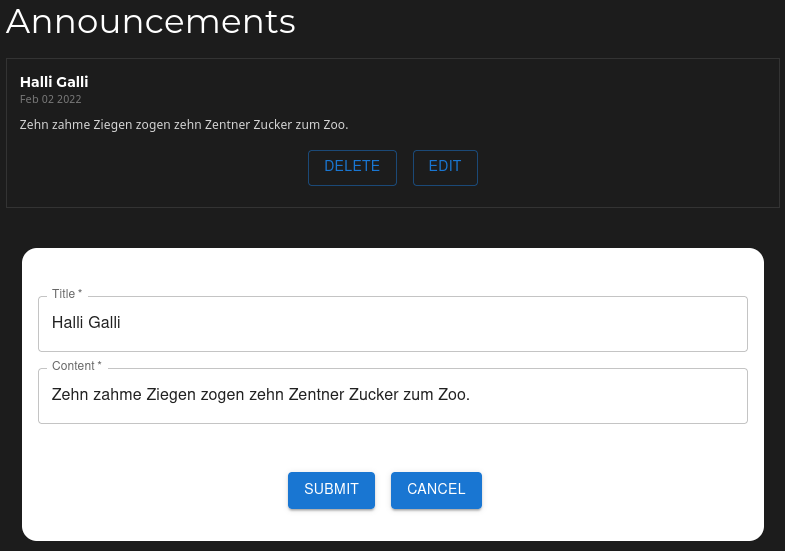
\includegraphics{images/announcement_edit.png}
\caption{Admin Announcement page}
\end{figure}\newpage

You can either create a very new announcement by filling out the text
fields in the announcement editor at the top of the page or you can edit
existing announcements to update or delete them.

\begin{figure}
\centering
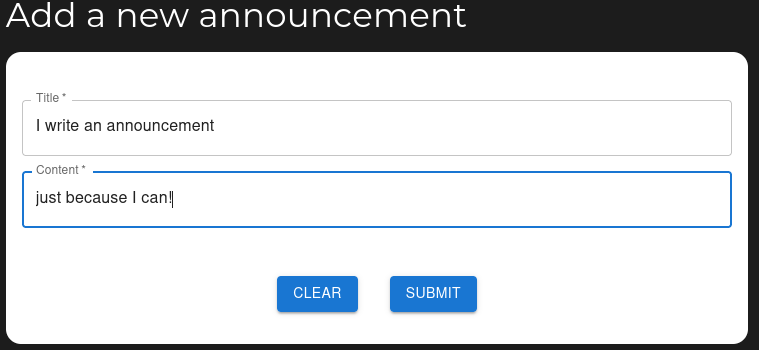
\includegraphics{images/create_new_announcement.png}
\caption{Admin new announcement}
\end{figure}\newpage

\hypertarget{backend---team-database-management}{%
\subsubsection{Backend - Team Database
Management}\label{backend---team-database-management}}

This section contains database operations in regards to the user teams.

\hypertarget{inviting-and-editing-admins-team}{%
\paragraph{Inviting and editing Admins
Team}\label{inviting-and-editing-admins-team}}

Admins can change Admin team associations by entering the email address
of a person for which an operation should be applied. Then click on
\texttt{SEARCH\ USER} button emphasized in blue.

\begin{figure}
\centering
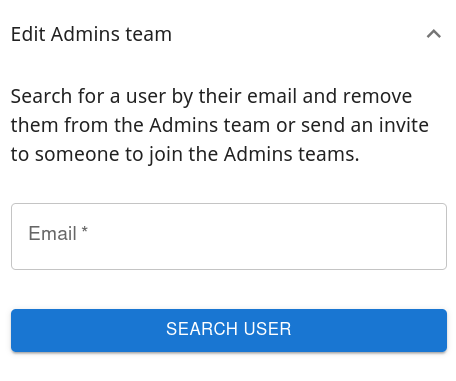
\includegraphics{images/adding_admins.png}
\caption{Add Admins}
\end{figure}

It will search for the email address in the database and based on the
result, it will suggest you to add the email address when not found, or
remove the email address when found. The email addresss acts as
represent for the account that is associated with it.

\begin{figure}
\centering
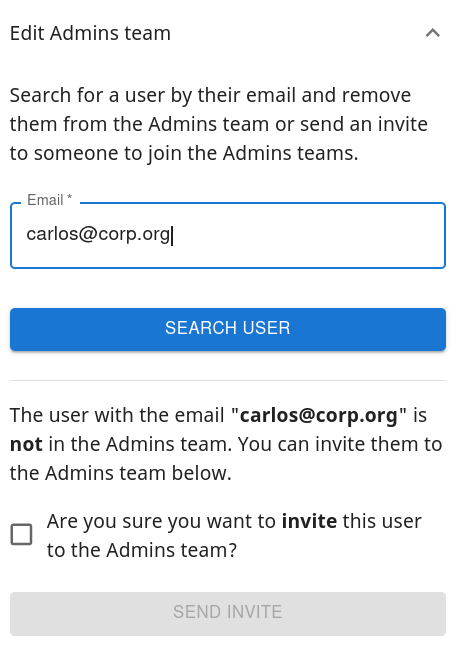
\includegraphics{images/invite_new_admin.png}
\caption{admin invitation}
\end{figure}\newpage

Before you can apply the operation, you first need to check the checkbox
for confirmation to prevent accidentally clicking on the button.

With an invitation, it will send an email to the provided email address,
notifying them about their invitation which they can accept.

You can also remove Admins, including yourself!

\begin{figure}
\centering
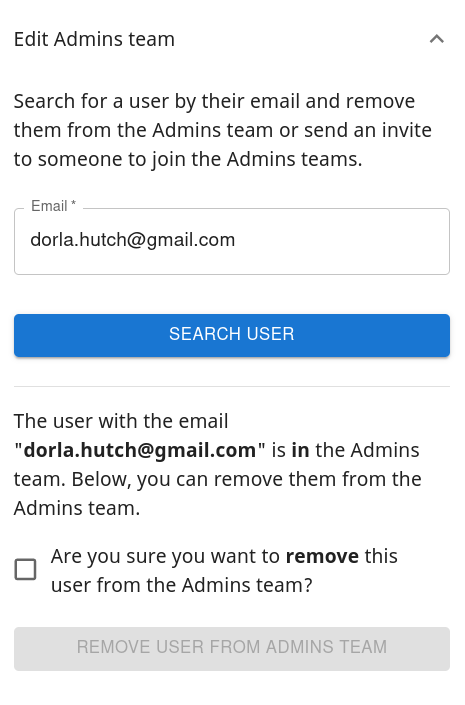
\includegraphics{images/remove_existing_admin.png}
\caption{admin removal}
\end{figure}\newpage

Let this be a lesson and don't invite people as Admins that could want
to grab for power and kick you from your Admin status!

\hypertarget{inviting-and-editing-partners-team}{%
\paragraph{Inviting and editing Partners
Team}\label{inviting-and-editing-partners-team}}

As a verified Partner and Admin, you can invite new partners. There is
no more powerful creature out there in ``NFT The World'' :-) .

Admins without Partner status cannot add new Partners to the database or
remove existing ones.

\begin{figure}
\centering
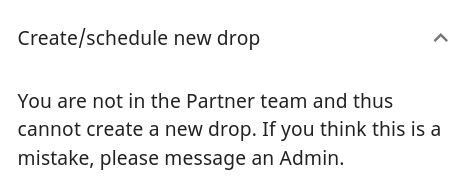
\includegraphics{images/admins_arent_partners.png}
\caption{Only Partners can manage Partners}
\end{figure}\newpage

Otherwise, as a partner, you can add new partners in the same way how
new Admins can be added.

\begin{figure}
\centering
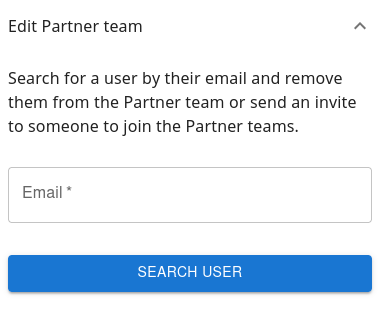
\includegraphics{images/add_partners.png}
\caption{Adding Partners}
\end{figure}\newpage

\hypertarget{contract---smart-contract-interaction}{%
\subsubsection{Contract - Smart Contract
interaction}\label{contract---smart-contract-interaction}}

In this section, special blockchain transactions can be initiated which
append live blockchain data. For security, the partners association is
saved directly on the blockchain.

\hypertarget{creating-an-nft-drop}{%
\paragraph{Creating an NFT Drop}\label{creating-an-nft-drop}}

Basically just a convenient shortcut for the additional profile button
which can be used by Partners with Admin status. Read more about NFT
Drop creation in the Partners Capabilities section.

\begin{figure}
\centering
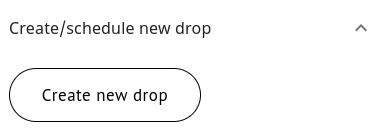
\includegraphics{images/drop_creation_admin_button.png}
\caption{NFT Drop Creation Admin Button}
\end{figure}

\hypertarget{adding-partnersadmins}{%
\paragraph{Adding Partners/Admins}\label{adding-partnersadmins}}

Well, actually every Admin can add Partners and thus themselves as well.

\begin{figure}
\centering
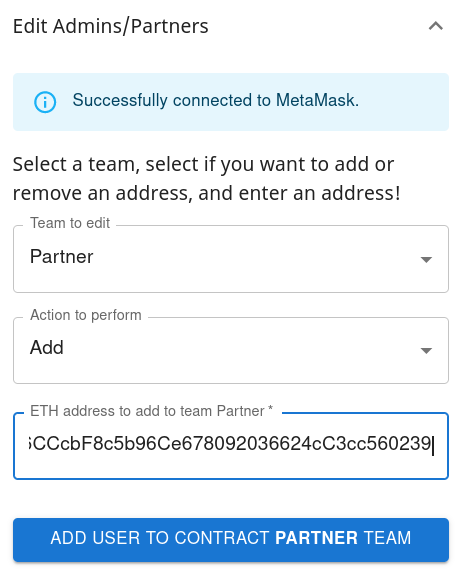
\includegraphics{images/Add_partner.png}
\caption{Add a partner}
\end{figure}\newpage

Select which team should be modified and below the operation to apply to
a (potential) team member.

Then enter the hexadecimal address of the wallet that should obtain
Partner status. A registered user logged in with that wallet will be
entitled to the capabilities of verified partners!

Click on the emphasized blue button saying
\texttt{ADD\ USER\ TO\ CONTRACT\ PARTNER\ TEAM} to conduct the
operation. Keep in mind that this is a blockchain transaction and
requires paying a gas fee. MetaMask will open and prompt you for
confirmation.

You can estimate the gas limit with \(30000\).

\end{document}
